\documentclass[springer.tex]{subfiles}
\graphicspath{ {./figures/} }

\begin{document}
\chapter{Debugging Programs}
\label{chap:testing}
A software bug is an error in a computer program that causes it to produce an incorrect result or behave in an unintended manner. The term 'bug' was used by Thomas Edison in 1878\footnote{\url{https://en.wikipedia.org/wiki/Software_bug}}\footnote{\url{http://edison.rutgers.edu/NamesSearch/DocImage.php3?DocId=LB003487}}, but made popular in computer science by Grace Hopper, who found a moth interfering with the electronic circuits of the Harward Mark II electromechanical computer and coined the term \idx{bug} for errors in computer programs. The original bug is shown in \Cref{fig:bug}.
\begin{figure}
  \centering
  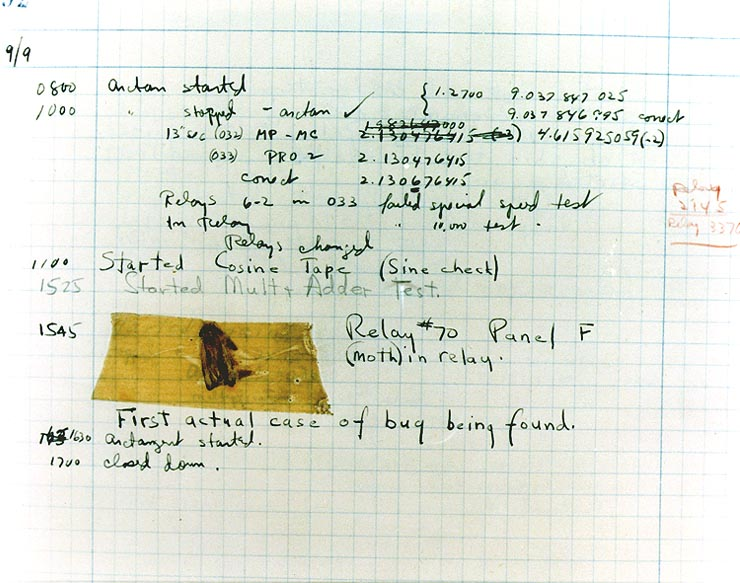
\includegraphics[width=0.45\linewidth]{H96566k}
  \caption{The first computer bug, caught by Grace Hopper, U.S. Naval Historical Center Online Library Photograph NH 96566-KN.}
  \label{fig:bug}
\end{figure}
Software is everywhere, and errors therein have a huge economic impact on our society and can threaten lives\footnote{\url{https://en.wikipedia.org/wiki/List_of_software_bugs}}.

Given code, which has been identified as erroneous, \idx{debugging} can begin. The cause of a bug can either be that the chosen algorithm is the wrong one for the job, or the implementation of it has an error. In the debugging process, we have to keep an open mind and not rely on assumptions. A frequent source of errors is that the state of a program is different than expected, e.g., because the calculation performed is different than intended, or that the return of a library function is different than expected. The most important tool for debugging is \emph{simplification}. This is similar to white-box testing, but where the units tested are very small. E.g., the suspected piece of code could be broken down into smaller functions or code snippets, which are given well-defined input, and, e.g., use \lstinline!printfn! statements to obtain the output of the code snippet. Another related technique is to use \idx{mockup code}, that is, replacing parts of the code with code that produces safe and relevant results. If the bug is not obvious, then more rigorous techniques must be used, such as \idx{tracing}. Some development interfaces have a built-in tracing system, will print inferred types and some binding values. However, often the source of a bug is due to a misunderstanding of the flow of data through a program execution, and we will in the following section introduce \idx{Trace by hand} as a technique to simulate the execution of a program by hand. In the following section, tracing will refer to the Trace by hand method.

The concept of Tracing by hand, will be developed throughout this book. Here we will concentrate in the basics, and as we introduce more complicated programming structures, we will develop the Tracing by hand accordingly. Tracing may seem tedious in the beginning, but in conjunction with strategically placed debugging \lstinline!printfn! statements, it is a very valuable tool for debugging.

Consider the program in \Cref{lexicalScopeTracing}.
%
\fs{lexicalScopeTracing}{Example of lexical scope and closure environment.}
%
The program calls \lstinline{testScope 2.0}, and by running the program, we see that the return-value is \lstinline{6.0} and not \lstinline{8.0}, as we had expected. Hence, we will use tracing to understand the result.

Tracing a program by hand means that we simulate its execution and, as part of that, keep track of the bindings, assignments closures, scopes, and input and output of the program. To do this, we need to consider the concept of \idx[environment]{environments}.

Environments describe bindings available to the program at the present scope and at a particular time and place in the code. There is always an outer environment, called $E_0$, and each time we call a function or create a scope, we create a new environment. Only one environment can be active at a time, and it is updated as we simulate the execution of code with new bindings and temporary evaluations of expressions. Once a scope is closed, then its environment is deleted and a return-value is transported to its enclosing environment. In tracing, we note return-values explicitely. Likewise, output from, e.g., \lstinline{printfn} is reported with a special notation.

To trace code, we make a table with 4 columns: Step, Line, Environment, and Bindings and evaluations. The Step column enumerates the steps performed. The Line column contains the program-line treated in a step {\em where} the present environment is updated. The Environment contains the name of the present environment, and Bindings $\ldots$ shows {\em what}  in the environment is updated.

The code in \Cref{lexicalScopeTracing} contains a function definition and a call, hence, the first lines of our table looks like,
\begin{quote}
  \begin{tabular*}{0.9\linewidth}{l|lll}
    Step & Line & Env.\ & Bindings and evaluations\\
    \hline
    0 & - & $E_0$ & ()\\
    1 &\ref{lexicalScopeTracing:testScope} & $E_0$ & $\text{testScope} = \big((x), \text{testScope-body}, ()\big)$\\
    2 &\ref{lexicalScopeTracing:print} & $E_0$ & $\text{testScope } 2.0 = \text{?}$
  \end{tabular*}
\end{quote}
The elements of the table is to be understood as follows. Step~0 initializes the outer environment. In order for us to remember that the environment is empty, we write the unit value \lexeme{()}. Reading the code from top to bottom, the first nonempty and non-comment line we meet is line~\ref{lexicalScopeTracing:testScope}, hence, in Step~1, we update the enviroment with the binding of a function to the name \lstinline{testScope}. Since functions are values in F\#, we note their bindings by their closures: a tuple of argument names, the function-body, and the values lexically available at the place of binding. See \Cref{sec:functions} for more information on closures. Following the function-binding, the \lstinline{printfn} statement is called in line~\ref{lexicalScopeTracing:print} to print the result \lstinline{testScope 2.0}. However, before we can produce any output, we must first evaluate \lstinline{testScope 2.0}. Since we do not yet know what this function evaluates to, in Step~2 we simply write the call with a question mark. The call causes the creation of a new environment, and we continue our table as follows,
\begin{quote}
  \begin{tabular*}{0.9\linewidth}{l|lll}
    Step & Line & Env.\ & Bindings and evaluations\\
    \hline
    3 & \ref{lexicalScopeTracing:testScope} & $E_1$ & $\big((x=2.0), \text{testScope-body}, ()\big)$
  \end{tabular*}
\end{quote}
This means that we are going to execute the code in testScope-body. The function was called with $2.0$ as argument, causing $x=2.0$. Hence, the only binding available at the start of this environment is to the name \lstinline{x}. In the testScope-body, we make 3 further bindings and a function call. First to \lstinline{a}, then to \lstinline{f}, then to another \lstinline{a}, which will overshadow the previous binding, and finally we call \lstinline{f}. Thus, our table is updated as follows,
\begin{quote}
  \begin{tabular*}{0.9\linewidth}{l|lll}
    Step & Line & Env.\ & Bindings and evaluations\\
    \hline
    4 & \ref{lexicalScopeTracing:a1} & $E_1$ & $a = 3.0$\\
    5 & \ref{lexicalScopeTracing:f} & $E_1$ & $\text{f} = \big((z), \text{a * z}, (a = 3.0, x = 2.0)\big)$\\
    6 & \ref{lexicalScopeTracing:a2} & $E_1$ & $a = 4.0$\\
    7 & \ref{lexicalScopeTracing:return} & $E_1$ & $\text{f } x = \text{?}$
  \end{tabular*}
\end{quote}
Note that by lexical scope, the closure of \lstinline!f! includes everything above its binding in $E_1$, and therefore we add $a = 3.0$ and $x = 2.0$ to the environment element in its closure. This has consequences for the following call to \lstinline!f! in line~\ref{lexicalScopeTracing:return}, which creates a new environment based on \lstinline{f}'s closure and the value of its arguments. The value of \lstinline{x} in Step~7 is found by looking in the previous steps for the last binding to the name \lstinline{x} in $E_1$, which occurs in Step~3. Note that the binding to a name \lstinline{x} in Step~5 is an internal binding in the closure of \lstinline{f} and is irrelevant here. Hence, we continue the table as,
\begin{quote}
  \begin{tabular*}{0.9\linewidth}{l|lll}
    Step & Line & Env.\ & Bindings and evaluations\\
    \hline
    8 & \ref{lexicalScopeTracing:f} & $E_2$ & $\big((z = 2.0), \text{a * z}, (a = 3.0, x = 2.0)\big)$
  \end{tabular*}
\end{quote}
Executing the body of \lstinline{f}, we initially have 3 bindings available: \lstinline{z = 2.0}, \lstinline{a = 3.0}, and \lstinline{x = 2.0}. Thus, to evaluate the expression \lstinline{a * z}, we use these bindings and write,
\begin{quote}
  \begin{tabular*}{0.9\linewidth}{l|lll}
    Step & Line & Env.\ & Bindings and evaluations\\
    \hline
    9 & \ref{lexicalScopeTracing:f} & $E_2$ & $a * z = 6.0$\\
    10 & \ref{lexicalScopeTracing:f} & $E_2$ & $\text{return} = 6.0$
  \end{tabular*}
\end{quote}
The 'return'-word is used to remind us that this is the value to replace the question mark with in Step~7. Here we will make a mental note and not physically replace the question mark with the calculated value. If you are ever in doubt which call is connected with which return value, seek upwards in the table from the return statement for the first question mark. Now we delete $E_2$ and return to the enclosing environment, $E_1$. Here the function call was the last expression, hence the return-value from \lstinline{testScope} will be equal to the return-value from \lstinline{f}, and we write,
\begin{quote}
  \begin{tabular*}{0.9\linewidth}{l|lll}
    Step & Line & Env.\ & Bindings and evaluations\\
    \hline
    11 & \ref{lexicalScopeTracing:f} & $E_1$ & return $= 6.0$
  \end{tabular*}
\end{quote}
Similarly, we delete $E_1$ and return to the question mark in Step~2, which is replaced by the value $6.0$. We can now finish the \lstinline{printfn} statement and produce the output,
\begin{quote}
  \begin{tabular*}{0.9\linewidth}{l|lll}
    Step & Line & Env.\ & Bindings and evaluations\\
    \hline
    12 & \ref{lexicalScopeTracing:print} & $E_0$ & output = ``6.0$\backslash$n'' 
  \end{tabular*}
\end{quote}
The return-value of a \lstinline{printfn} statement is \lstinline{()}, and since this line is the last of our program, we return \lstinline{()} and end the program:
\begin{quote}
  \begin{tabular*}{0.9\linewidth}{l|lll}
    Step & Line & Env.\ & Bindings and evaluations\\
    \hline
    13 &\ref{lexicalScopeTracing:print} & $E_0$ & $\text{return} = ()$
  \end{tabular*}
\end{quote}
The full table is shown for completeness in \Cref{tab:tracingFunctions}.
\begin{table}
  \centering
  \fbox{
  \begin{tabular*}{0.9\linewidth}{l|lll}
    Step & Line & Env.\ & Bindings and evaluations\\
    \hline
    0 & - & $E_0$ & ()\\
    1 &\ref{lexicalScopeTracing:testScope} & $E_0$ & $\text{testScope} = \big((x), \text{testScope-body}, ()\big)$\\
    2 &\ref{lexicalScopeTracing:print} & $E_0$ & $\text{testScope } 2.0 = \text{?}$\\
    3 & \ref{lexicalScopeTracing:testScope} & $E_1$ & $\big((x=2.0), \text{testScope-body}, ()\big)$\\
    4 & \ref{lexicalScopeTracing:a1} & $E_1$ & $a = 3.0$\\
    5 & \ref{lexicalScopeTracing:f} & $E_1$ & $\text{f} = \big((z), \text{a * z}, (a = 3.0, x = 2.0)\big)$\\
    6 & \ref{lexicalScopeTracing:a2} & $E_1$ & $a = 4.0$\\
    7 & \ref{lexicalScopeTracing:return} & $E_1$ & $\text{f } x = \text{?}$\\
    8 & \ref{lexicalScopeTracing:f} & $E_2$ & $\big((z = 2.0), \text{a * z}, (a = 3.0, x = 2.0)\big)$\\
    9 & \ref{lexicalScopeTracing:f} & $E_2$ & $a * z = 6.0$\\
    10 & \ref{lexicalScopeTracing:f} & $E_2$ & $\text{return} = 6.0$\\
    11 & \ref{lexicalScopeTracing:f} & $E_1$ & return $= 6.0$\\
    12 & \ref{lexicalScopeTracing:print} & $E_0$ & output = ``6.0$\backslash$n'' \\
    13 &\ref{lexicalScopeTracing:print} & $E_0$ & $\text{return} = ()$\\
  \end{tabular*}
  }
\caption{The complete table produced while tracing the program in \Cref{lexicalScopeTracing} by hand.}
\label{tab:tracingFunctions}
\end{table}
Hence, we conclude that the program outputs the value \lstinline{6.0}, since the function \lstinline{f} uses the first binding of \lstinline{a = 3.0}, and this is because the binding of \lstinline{f} to the expression \lstinline{a * z} creates a closure with a lexical scope. Thus, in spite that there is an overshadowing value of \lstinline{a}, when \lstinline{f} is called, this binding is ignored in the body of \lstinline{f}. To correct this, we update the code as shown in \Cref{lexicalScopeTracingCorrected}.
%
\fs{lexicalScopeTracingCorrected}{Tracing the code in \Cref{lexicalScopeTracing} by hand produced the table in \Cref{tab:tracingFunctions}, and to get the desired output, we correct the code as shown here.}
%


\end{document}
